%%%%%%%%%%%%%%%%%%%%%%%%%%%%%%%%%%%%
%% Template file SP 2024
%% Include in directory homework.sty and headerfooter.tex
%%%%%%%%%%%%%%%%%%%%%%%%%%%%%%%%%%%%

\documentclass[12pt]{article}
\usepackage{homework}

\graphicspath{{images/}}
\geometry{letterpaper, portrait, includeheadfoot=true, hmargin=1in, vmargin=1in}

\setcounter{section}{-1}
%% Solution hiding %%
\usepackage[utf8]{inputenc}
\usepackage{lipsum}


\begin{document}
\singlespacing

\renewcommand{\familydefault}{\rmdefault}
\pagestyle{fancy}
\fancyhf{}
\setlength{\headheight}{30pt}
\renewcommand{\headrulewidth}{0.4pt}
\renewcommand{\footrulewidth}{0.4pt}
\lhead{\large Homework 2 \\ Due Feb. 20, 2024 }
\rhead{\large CS 446 \\ Spring 2024}
\rfoot{\textbf{Page \thepage}}
\lfoot{}

\section{Instructions}

Homework is due Tuesday, April 30, 2024 at 23:59pm Central Time.
Please refer to \url{https://courses.grainger.illinois.edu/cs446/sp2024/homework/hw/index.html} for course policy on homeworks and submission instructions.

\section{Bellman Equation}
\subsection{}
\begin{eqnarray}
    Q^{\pi}(s, a) = R(s_0=s, a_0=a) + \sum_{t=0}^{\infty } \mathbb{E} _{a_{t+1} \sim  \pi (a_{t+1}|s_{t+1})
                                            \atop
                                           s_{t+1} \sim p(s_{t+1}|s_t , a_t) } [\gamma^{t+1} R(s_{t+1} , a_{t+1})] \nonumber
\end{eqnarray}

\subsection{}
\begin{eqnarray}
    Q^{\pi}(s, a) &=& R(s_0=s, a_0=a) + \sum_{t=0}^{\infty } \mathbb{E} _{a_{t+1} \sim  \pi (a_{t+1}|s_{t+1})
                                            \atop
                                           s_{t+1} \sim p(s_{t+1}|s_t , a_t) } [\gamma^{t+1} R(s_{t+1} , a_{t+1})] \nonumber \\
    &=& R(s_0, a_0) + \gamma \sum_{s_1} p(s_1 | s_0, a_0) \sum_{a_1} \pi(a_1 | s_1) \nonumber  \\
    && \quad  \quad \quad \quad\{R(s_1, a_1) +\sum_{t=1}^{\infty } \mathbb{E} _{a_{t+1} \sim  \pi (a_{t+1}|s_{t+1}) \atop s_{t+1} \sim p(s_{t+1}|s_t , a_t) } [\gamma^{t+1} R(s_{t+1} , a_{t+1})]\} \nonumber \\
    &=& R(s_0, a_0) + \gamma \sum_{s_1} p(s_1 | s_0, a_0) \sum_{a_1} \pi(a_1 | s_1) Q^{\pi}(s_1, a_1) \nonumber
\end{eqnarray}

\subsection{}
\begin{eqnarray}
    Q(s , a) \leftarrow Q(s , a) + \alpha \left[ R(s, a) + \gamma \max_{a'} Q(s' , a') - Q(s , a) \right] \nonumber
\end{eqnarray}

\subsection{}
If for every steps, the reward is the maximum reward, then the Q-value will be the maximum reward. In this case, 
\begin{equation}
    \max Q* = R_{max} + \gamma R_{max} + \gamma^2 R_{max} + \cdots = \frac{R_{max}}{1 - \gamma} \nonumber
\end{equation}

\subsection{}
(a)\begin{equation}
    Q(s_1 , a_1) = 0 + 0.5 * (-10 + 0.5 * 0 - 0) = -5 \nonumber
\end{equation}

(b)\begin{equation}
    Q(s_1 , a_2) = 0 + 0.5 * (-10 + 0.5 * 0 - 0) = -5 \nonumber
\end{equation}

(c)\begin{equation}
    Q(s_2 , a_1) = 0 + 0.5 * (18.5 + 0.5 * (-5) - 0) = 8 \nonumber
\end{equation}

(d)\begin{equation}
    Q(s_1, a_2) = -5 + 0.5 * (-10 + 0.5 * 8 + 5 ) = -5.5  \nonumber
\end{equation}

\newpage

\section{Combination Lock}
\subsection{}
Denotes $N_{s_i}$ as the expected number of steps from state 1 to state i. Easily, we have $ N_{s_1} = 0$. Then, we have following equations:
\begin{align*}
    N_{s_2} &= 0.5*(N_{s_1}+1) + 0.5*(N_{s_1} + 1 + N_{s_2}) \\
            &= N_{s_1} + 1 + 0.5N_{s_2} \\
    \Rightarrow N_{s_2} &= 2 N_{s_1} + 2 
\end{align*}

Similarly, we have,
\begin{align*}
    N_{s_3} &= 0.5*(N_{s_2}+1) + 0.5*(N_{s_2} + 1 + N_{s_3}) \\
    \Rightarrow N_{s_3} &= 2 N_{s_2} + 2 \\
    &\vdots \\
    N_{s_n} &= 2N_{s_{n-1}}+2
\end{align*}

Iteratively substitute $N_{s_{i}}$ into $N_{s_{i+1}}$, we get,
\begin{align*}
    N_{s_n} &= 2N_{s_{n-1}} + 2\\
    &= 2(2N_{s_{n-2}} + 2) + 2 \\
    &= 2^2N_{s_{n-2}} + 2^2 + 2 \\
    &\vdots \\
    &= 2^{n-1}N_{s_1} + 2^{n-1} + 2^{n-2} + \cdots + 2^2 + 2 \\
    &= 2^{n-1} + 2^{n-2} + \cdots + 2^2 + 2 = 2^n - 2
\end{align*}

\subsection{}
We have following equations:
    \begin{align*}
        Q(s_n,a_1) &= 1 + \frac{\gamma}{2}(Q(s_n,a_1)+Q(s_n,a_2)) \\
                & = 1 + \gamma * \frac{1}{2} +\gamma^2 * \frac{1}{2} + \cdots \\
                & = 1 + \frac{\gamma}{2(1-\gamma)}\\
        Q(s_n,a_2) &= \frac{\gamma}{2}(Q(s_n,a_1)+Q(s_n,a_2))\\
                & = \frac{\gamma}{2(1-\gamma)} \\
        Q(s_{i},a_1) &= \frac{\gamma}{2}(Q(s_{i+1},a_1)+Q(s_{i+1},a_2))\\
        Q(s_{i},a_2) &= \frac{\gamma}{2}(Q(s_1,a_1)+Q(s_1,a_2))
    \end{align*}

    Iteratively substitute from step n to step 1,  we have,
    \begin{eqnarray*}
        Q(s_{n-1}, a_1) &=& \frac{\gamma}{2} (1 + \frac{\gamma}{2(1-\gamma)} + \frac{\gamma}{2(1-\gamma)}) \\
         &=& \frac{\gamma}{2}(1+\frac{\gamma}{1-\gamma}) = \frac{\gamma}{2(1-\gamma)}\\
         Q(s_{n-1}, a_2) &=& \frac{\gamma}{2}(Q(s_1,a_1)+Q(s_1,a_2))\\
         Q(s_{n-2},a_1) &=&\frac{\gamma}{2} (\frac{\gamma}{2(1-\gamma)} + \frac{\gamma}{2}(Q(s_1,a_1)+Q(s_1,a_2)))\\
            &=& (\frac{\gamma}{2})^2\frac{1}{(1-\gamma)} + (\frac{\gamma}{2})^2((Q(s_1,a_1)+Q(s_1,a_2)))\\
        Q(s_{n-2}, a_2) &=& \frac{\gamma}{2}(Q(s_1,a_1)+Q(s_1,a_2))\\
        Q(s_{n-3}, a_1) &=& (\frac{\gamma}{2})^3\frac{1}{(1-\gamma)} + (\frac{\gamma}{2})^3((Q(s_1,a_1)+Q(s_1,a_2)))
        +(\frac{\gamma}{2})^2((Q(s_1,a_1)+Q(s_1,a_2)))\\
        Q(s_{n-3}, a_2) &=& \frac{\gamma}{2}(Q(s_1,a_1)+Q(s_1,a_2))\\
        &\vdots\\
        Q(s_{i}, a_1) &=& (\frac{\gamma}{2})^{n-i}\frac{1}{(1-\gamma)} + (\frac{\gamma}{2})^{n-i}(Q(s_1,a_1)+Q(s_1,a_2)) + \cdots + (\frac{\gamma}{2})^{2}((Q(s_1,a_1)+Q(s_1,a_2)))\\
        &=&  (\frac{\gamma}{2})^{n-i}\frac{1}{(1-\gamma)} + (\frac{\gamma(1- (\frac{\gamma}{2})^{n-1-i})}{2-\gamma})(Q(s_1,a_1)+Q(s_1,a_2))
    \end{eqnarray*}
    We can then derive the similar equation for $Q_(s_{1}, a_1)$:
    \begin{eqnarray*}
        Q(s_1,a_1) &=& (\frac{\gamma}{2})^{n-1}\frac{1}{(1-\gamma)} + (\frac{\gamma(1- (\frac{\gamma}{2})^{n-2})}{2-\gamma})(Q(s_1,a_1)+Q(s_1,a_2))
    \end{eqnarray*}
    Since we know $Q(s_1,a_2) = \frac{\gamma}{2}(Q(s_1, a_1) + Q(s_1, a_2))$, we can solve for $Q(s_1,a_1)$:
    \begin{eqnarray*}
        Q(s_1,a_1) &=& (\frac{\gamma}{2})^{n-1}\frac{1}{(1-\gamma)} + (\frac{\gamma(1- (\frac{\gamma}{2})^{n-2})}{2-\gamma})(Q(s_1,a_1)+Q(s_1,a_2)) \\
        &=& (\frac{\gamma}{2})^{n-1}\frac{1}{(1-\gamma)} + (\frac{\gamma(1- (\frac{\gamma}{2})^{n-2})}{2-\gamma})(\frac{2}{2-\gamma}) Q(s_1,a_1)\\
    \end{eqnarray*}

    The solution to the above equation is:
    \begin{equation}
        Q(s_1,a_1)= (\frac{\gamma}{2})^{n}\frac{1}{(1-\gamma)} \frac{1}{(1-\frac{2\gamma(1- (\frac{\gamma}{2})^{n-2})}{(2-\gamma)^2})} \nonumber
    \end{equation}
    Thus, we can write out the closed form solution for all state:
    \begin{align*}
        Q(s_1,a_1)&= (\frac{\gamma}{2})^{n}\frac{1}{(1-\gamma)} \frac{1}{(1-\frac{2\gamma(1- (\frac{\gamma}{2})^{n-2})}{(2-\gamma)^2})} \\
        Q(s_1,a_2)&= \frac{\gamma}{2-\gamma}Q(s_1, a_1)\\
        Q(s_{i}, a_1) &=  (\frac{\gamma}{2})^{n-i}\frac{1}{(1-\gamma)} + (\frac{\gamma(1- (\frac{\gamma}{2})^{n-1-i})}{2-\gamma})(Q(s_1,a_1)+Q(s_1,a_2))\\
        Q(s_{i}, a_2) &= \frac{\gamma}{2}(Q(s_1, a_1) + Q(s_1, a_2)) \\
        Q(s_n,a_1) &= 1 + \frac{\gamma}{2(1-\gamma)} \\
        Q(s_n,a_2) &= \frac{\gamma}{2(1-\gamma)}
    \end{align*}

\subsection{}
k-1 steps. From the results above, we can easily see $Q(s_n, a_1) > Q(s_n, a_2)$ and $Q(s_1, a_1) > Q(s_1, a_2)$. For states between 1 and n, let's consider the difference between $Q(s_i, a_1)$ and $Q(s_i, a_2)$:
\begin{eqnarray*}
    Q(s_{i}, a_1) - Q(s_{i}, a_2) &=& (\frac{\gamma}{2})^{n-i}\frac{1}{(1-\gamma)} + (\frac{\gamma(1- (\frac{\gamma}{2})^{n-1-i})}{2-\gamma}-\frac{\gamma}{2})(Q(s_1,a_1)+Q(s_1,a_2))\\
    &=& (\frac{\gamma}{2})^{n-i}\frac{1}{(1-\gamma)} + (\frac{\gamma(1- (\frac{\gamma}{2})^{n-1-i})}{2-\gamma}-\frac{\gamma}{2})(Q(s_1,a_1)+Q(s_1,a_2))\\
    &\ge& 0 
\end{eqnarray*}

\newpage

\section{Q-value Initialization}
\subsection{}
As the same as question 2.1. Since all Q values are initialized to the same values for both policies, they will choose random actions at each state. The expected number of steps to reach the final state is $2^n - 2$.

\subsection{}
Since all Q values are initialized to 0 for policy 1, so the Q values will remain 0 before reaching the final state, which again downgrades to random policy. The expected number of steps to reach the final state is still $2^n - 2$.

\subsection{}
Still $2^n - 2$. Because we didn't update any Q values for states before final state.

\subsection{}
If we have replay buffer that stores previous transitions, for example $(s_{n-1}, a_1, s_{n})$, after updating $Q(s_n, a_1)$, we can immediately update $Q(s_{n-1}, a_1)$ using the stored transition from replay buffer. 

\subsection{}
n-1 steps. At each state, the agent randomly takes $a_1$ to move, and the updated Q values won't affect the agent's decision on future states. In this case, the minimum steps is $n-1$.
\newpage

\section{Policy Gradient}
\subsection{}
\begin{eqnarray}
    \nabla J(\theta) &=& \nabla \mathbb{E}_{\tau \sim \pi_{\theta}} [R(\tau)] \nonumber \\
    &=& \mathbb{E} _{\tau \sim \pi_{\theta}}[R(\tau) \nabla \log \pi_{\theta}(\tau)] \nonumber \\
    &=& \mathbb{E} _{\tau \sim \pi_{\theta}} [R(\tau) \nabla \log d_0(s_0) \prod_{i=0}^{T-1} \pi_{\theta}(a_i | s_i) p(s_{i+1} | s_i, a_i) \pi(a_T | s_T) ] \nonumber \\
    &=& \mathbb{E} _{\tau \sim \pi_{\theta}} [ R(\tau) \nabla \sum_{i=0}^{T-1} \log \pi_{\theta}(a_i | s_i)] \nonumber
\end{eqnarray}


\subsection{}
\begin{eqnarray}
    \nabla J(\theta) &=& \nabla \mathbb{E}_{s \sim d_0} [V ^{\pi_{\theta}}(s)] \nonumber \\
    &=& \mathbb{E}_{s \sim d_0} [\nabla V ^{\pi_{\theta}}(s)] \nonumber \\
    &=& \mathbb{E} _{s \sim d_0} \nabla \sum_{a} \pi_{\theta}(a | s) Q^{\pi_{\theta}}(s, a) \nonumber \\
    &=& \mathbb{E} _{s \sim d_0} \sum_{a} (\nabla \pi_{\theta}(a | s) Q^{\pi_{\theta}}(s, a) + \pi_{\theta}(a | s)\nabla Q^{\pi_{\theta}}(s, a) )\nonumber
\end{eqnarray}
where we konw that $ Q^{\pi_{\theta}}(s, a) = R(s, a) + \gamma \sum_{s'} p(s' | s, a) V^{\pi_{\theta}}(s')$ and $R(s, a)$ is independent of $\theta$, we have
\begin{eqnarray}
    \nabla J(\theta) &=& \mathbb{E} _{s \sim d_0} \sum_{a} (\nabla \pi_{\theta}(a | s) Q^{\pi_{\theta}}(s, a) + \pi_{\theta}(a | s) \gamma \sum_{s'} p(s' | s, a)\nabla V^{\pi_{\theta}}(s')) \nonumber \\
    &=& \mathbb{E} _{s \sim d_0 \atop a \sim \pi_{\theta}} \nabla \pi_{\theta}(a | s) Q^{\pi_{\theta}}(s, a) + \mathbb{E} _{s \sim d_0} \pi_{\theta}(a | s) \gamma \sum_{s'} p(s' | s, a)\nabla V^{\pi_{\theta}}(s') \nonumber \\
    &=& \mathbb{E} _{s \sim d_0 \atop a \sim \pi_{\theta}} \nabla \pi_{\theta}(a | s) Q^{\pi_{\theta}}(s, a) + \mathbb{E} _{s' \sim d_1 \atop a \sim \pi_{\theta}} \gamma \nabla V^{\pi_{\theta}}(s') \nonumber
\end{eqnarray}

Then, we iteratively substitute 
\begin{equation}
    \mathbb{E} _{s' \sim d_i \atop a \sim \pi_{\theta}} \nabla V^{\pi_{\theta}}(s') = \mathbb{E} _{s' \sim d_i \atop a \sim \pi_{\theta}} \nabla \pi_{\theta}(a | s) Q^{\pi_{\theta}}(s, a) + \mathbb{E} _{s' \sim d_{1+1} \atop a \sim \pi_{\theta}} \gamma \nabla V^{\pi_{\theta}}(s')
\end{equation}
     into the equation. We get,
\begin{eqnarray}
    \nabla J(\theta) &=& \mathbb{E} _{s \sim d_0 \atop a \sim \pi_{\theta}} \nabla \pi_{\theta}(a | s) Q^{\pi_{\theta}}(s, a) + \mathbb{E} _{s \sim d_1 \atop a \sim \pi_{\theta}} \gamma \nabla \pi_{\theta}(a | s) Q^{\pi_{\theta}}(s, a) + \cdots \nonumber \\
    &&\quad \quad \quad\quad \quad \quad\quad\quad + \mathbb{E} _{s \sim d_i \atop a \sim \pi_{\theta}} \gamma^i \nabla \pi_{\theta}(a | s) Q^{\pi_{\theta}}(s, a) + \cdots \nonumber \\
    &=&\sum_{s} \sum_{i=0}^{\infty} \gamma^i d_{i}\sum_{a}\pi_{\theta}(a | s) \nabla \pi_{\theta}(a | s) Q^{\pi_{\theta}}(s, a) \nonumber \\
    &=&  \mathbb{E} _{a  \sim \pi_{\theta} \atop s \sim d} \nabla \pi_{\theta}(a | s) Q^{\pi_{\theta}}(s, a) \nonumber
\end{eqnarray}

\subsection{}
We only need to show that $\mathbb{E}_{s \sim d \atop a \sim \pi_{\theta}} [f(s) \nabla_\theta \log \pi_{\theta}(a | s)] = 0 $.
\begin{eqnarray}
    \mathbb{E}_{s \sim d \atop a \sim \pi_{\theta}} [f(s) \nabla_\theta \log \pi_{\theta}(a | s)] &=& \sum_{s} d^\pi(s) f(s) \mathbb{E}_{a \sim \pi_\theta} \frac{1}{\pi_{\theta}(a | s)}\nabla \pi_\theta (a|s) \nonumber \\
    &=& \sum_{s} d^\pi(s) f(s) \sum_{a} \pi_{\theta}(a | s) * \frac{1}{\pi_{\theta}(a | s)} \nabla \pi_{\theta}(a | s) \nonumber \\
    &=& \sum_{s} d^\pi(s) f(s) \nabla \sum_{a} \pi_{\theta}(a | s) \nonumber \\
    &=& \sum_{s} d^\pi(s) f(s) \nabla 1 \nonumber \\
    &=& 0 \nonumber
\end{eqnarray}


\newpage

\section{Coding: Tabular Q-learning}
\subsection{}
\begin{enumerate}
    \item States correspond to observations in gym environments. In the case of "Taxi-v3", there are 500 discrete states. The action space is the set of actions that the agent can take for each state. Here, the action space is a discrete set of 6 actions.
    \item env.step() returns observation, reward, terminated, info and done. env.reset() returns observation and info. Each state is represented by a tuple: taxi\_row, taxi\_col, passenger\_location, destination, where each element is an integer.
    \item There are 4 render modes: 'human', 'rgb\_array', 'rgb\_array\_list' and 'ansi'. 'human' mode returns None and is only used for human display. 'rgb\_array' mode returns an numpy array representing the frame of the current state. 'rgb\_array\_list' mode returns a list of numpy arrays representing the frames since last reset. 'ansi' mode returns a terminal-style text representation of the current state.
    \item They use self.decode(self.s) to decode the current state into terminal texts. 
\end{enumerate}

% Code should be submitted on gradescope, there is no autograder
\subsection{}
\begin{figure}[H]
    \centering
    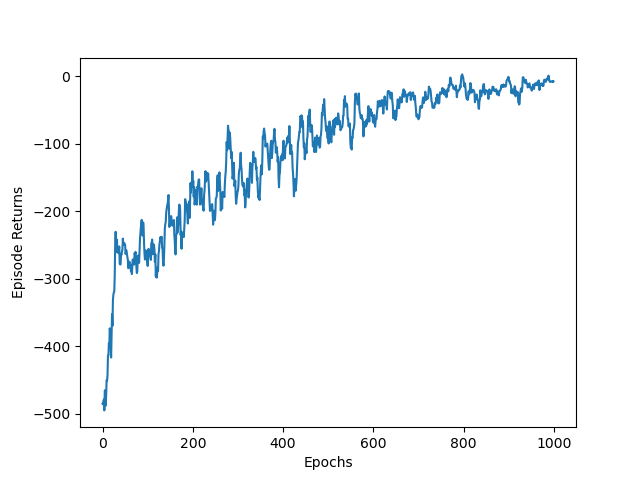
\includegraphics[width=0.8\textwidth]{imgs/q2.png}
    \caption{5.2 train rewards}
\end{figure}

\subsection{}
The success rate became very low (only 0.0427). Because the agent now is hard to learn the optimal Q values given the episodes. Thus, it is also hard to find the optimal policy.
\begin{figure}[H]
    \centering
    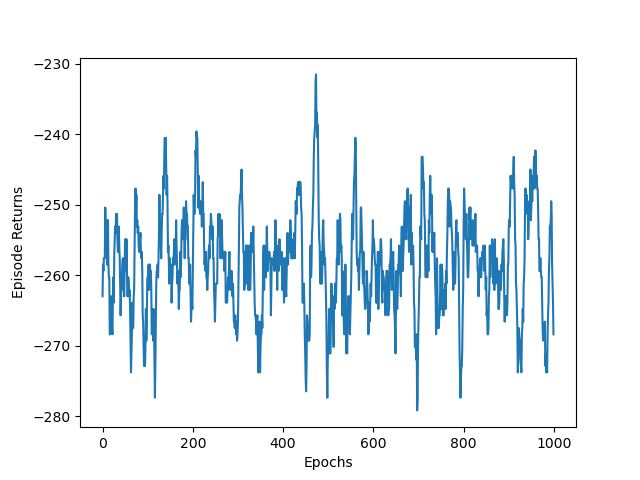
\includegraphics[width=0.8\textwidth]{imgs/q3.png}
    \caption{5.3 train rewards}
\end{figure}

\subsection{}
0.0427.
\begin{figure}[H]
    \centering
    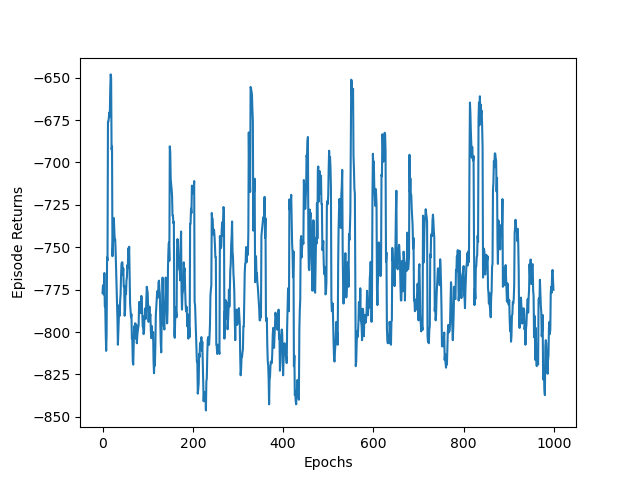
\includegraphics[width=0.8\textwidth]{imgs/q4.png}
    \caption{5.4 train rewards}
\end{figure}

\subsection{}
\begin{figure}[H]
    \centering
    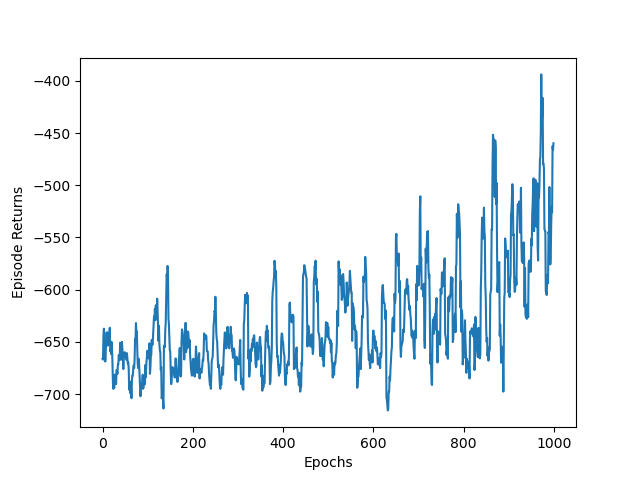
\includegraphics[width=0.8\textwidth]{imgs/q5.png}
    \caption{5.5 train rewards}
\end{figure}

\subsection{}
0.139.
\begin{figure}[H]
    \centering
    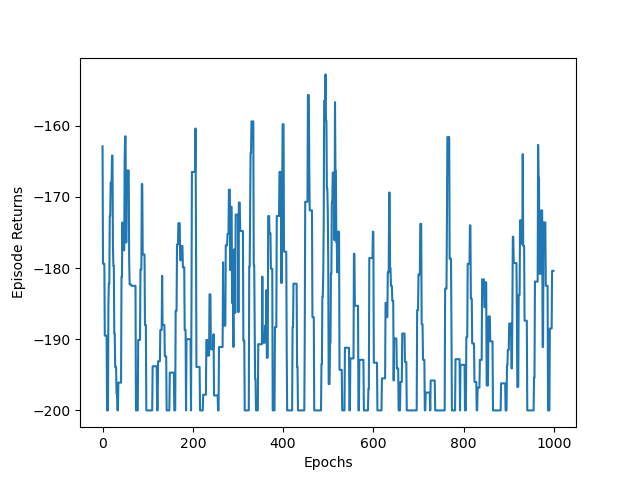
\includegraphics[width=0.8\textwidth]{imgs/q6.png}
    \caption{5.6 train rewards}
\end{figure}

\subsection{}
\begin{figure}[H]
    \centering
    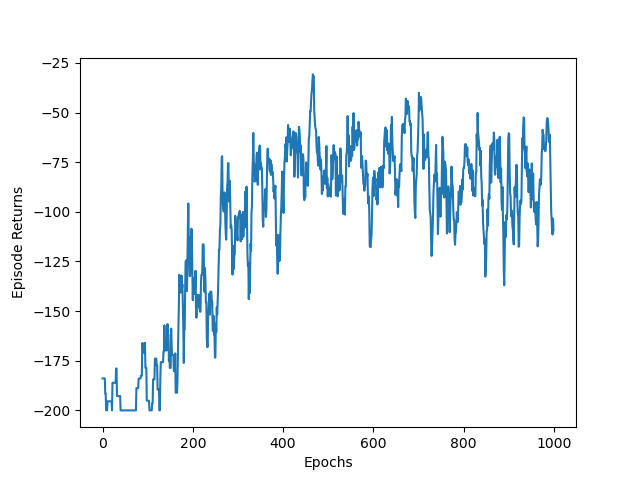
\includegraphics[width=0.8\textwidth]{imgs/q7.png}
    \caption{5.7 train rewards}
\end{figure}
\end{document}